%%%%%%%%%%%%%%%%%%%%%%%%%%%%%%%%%%%%%%%%%%%%%%%%%%%%%%%%%%%%%%%%%%%%%%
%%  Copyright by Wenliang Du.                                       %%
%%  This work is licensed under the Creative Commons                %%
%%  Attribution-NonCommercial-ShareAlike 4.0 International License. %%
%%  To view a copy of this license, visit                           %%
%%  http://creativecommons.org/licenses/by-nc-sa/4.0/.              %%
%%%%%%%%%%%%%%%%%%%%%%%%%%%%%%%%%%%%%%%%%%%%%%%%%%%%%%%%%%%%%%%%%%%%%%

\newcommand{\commonfolder}{../../common-files}

\documentclass[11pt]{article}

\usepackage[most]{tcolorbox}
\usepackage{times}
\usepackage{epsf}
\usepackage{epsfig}
\usepackage{amsmath, alltt, amssymb, xspace}
\usepackage{wrapfig}
\usepackage{fancyhdr}
\usepackage{url}
\usepackage{verbatim}
\usepackage{fancyvrb}
\usepackage{adjustbox}
\usepackage{listings}
\usepackage{color}
\usepackage{subfigure}
\usepackage{cite}
\usepackage{sidecap}
\usepackage{pifont}
\usepackage{mdframed}
\usepackage{textcomp}
\usepackage{enumitem}
\usepackage{hyperref}


% Horizontal alignment
\topmargin      -0.50in  % distance to headers
\oddsidemargin  0.0in
\evensidemargin 0.0in
\textwidth      6.5in
\textheight     8.9in 

\newcommand{\todo}[1]{
\vspace{0.1in}
\fbox{\parbox{6in}{TODO: #1}}
\vspace{0.1in}
}


\newcommand{\unix}{{\tt Unix}\xspace}
\newcommand{\linux}{{\tt Linux}\xspace}
\newcommand{\minix}{{\tt Minix}\xspace}
\newcommand{\ubuntu}{{\tt Ubuntu}\xspace}
\newcommand{\setuid}{{\tt Set-UID}\xspace}
\newcommand{\openssl} {\texttt{openssl}}


\pagestyle{fancy}
\lhead{\bfseries SEED Labs}
\chead{}
\rhead{\small \thepage}
\lfoot{}
\cfoot{}
\rfoot{}


\definecolor{dkgreen}{rgb}{0,0.6,0}
\definecolor{gray}{rgb}{0.5,0.5,0.5}
\definecolor{mauve}{rgb}{0.58,0,0.82}
\definecolor{lightgray}{gray}{0.90}


\lstset{%
  frame=none,
  language=,
  backgroundcolor=\color{lightgray},
  aboveskip=3mm,
  belowskip=3mm,
  showstringspaces=false,
%  columns=flexible,
  basicstyle={\small\ttfamily},
  numbers=none,
  numberstyle=\tiny\color{gray},
  keywordstyle=\color{blue},
  commentstyle=\color{dkgreen},
  stringstyle=\color{mauve},
  breaklines=true,
  breakatwhitespace=true,
  tabsize=3,
  columns=fullflexible,
  keepspaces=true,
  escapeinside={(*@}{@*)}
}

\newcommand{\newnote}[1]{
\vspace{0.1in}
\noindent
\fbox{\parbox{1.0\textwidth}{\textbf{Note:} #1}}
%\vspace{0.1in}
}


%% Submission
\newcommand{\seedsubmission}{
Debe enviar un informe de laboratorio detallado, con capturas de pantalla, para describir lo que ha hecho y lo que ha observado.
También debe proporcionar una explicación a las observaciones que sean interesantes o sorprendentes.
Enumere también los fragmentos de código más importantes seguidos de una explicación. No recibirán créditos aquellos fragmentos de códigos que no sean explicados.}

%% Book
\newcommand{\seedbook}{\textit{Computer \& Internet Security: A Hands-on Approach}, 2nd
Edition, by Wenliang Du. Para más detalles \url{https://www.handsonsecurity.net}.\xspace}

%% Videos
\newcommand{\seedisvideo}{\textit{Internet Security: A Hands-on Approach},
by Wenliang Du. Para más detalles \url{https://www.handsonsecurity.net/video.html}.\xspace}

\newcommand{\seedcsvideo}{\textit{Computer Security: A Hands-on Approach},
by Wenliang Du. Para más detalles \url{https://www.handsonsecurity.net/video.html}.\xspace}

%% Lab Environment
\newcommand{\seedenvironment}{Este laboratorio ha sido testeado en nuestra imagen pre-compilada de una VM con Ubuntu 16.04, que puede ser descargada del sitio oficial de SEED.\xspace}

\newcommand{\seedenvironmentA}{Este laboratorio ha sido testeado en nuestra imagen pre-compilada de una VM con Ubuntu 16.04, que puede ser descargada del sitio oficial de SEED.\xspace}

\newcommand{\seedenvironmentB}{Este laboratorio ha sido testeado en nuestra imagen pre-compilada de una VM con Ubuntu 20.04, que puede ser descargada del sitio oficial de SEED .\xspace}

\newcommand{\seedenvironmentC}{Este laboratorio ha sido testeado en nuestra imagen pre-compilada de una VM con Ubuntu 20.04, que puede ser descargada del sitio oficial de SEED. Sin embargo, la mayoría de nuestros laboratorios pueden ser realizados en la nube para esto Ud. puede leer nuestra guía que explica como crear una VM de SEED en la nube.\xspace}

\newcommand{\seedenvironmentAB}{
Este laboratorio ha sido testeado en nuestras imagenes pre-compiladas de una VM con Ubuntu 16.04 y otra con Ubuntu 20.04, que pueden ser descargadas del sitio oficial de SEED.\xspace}

\newcommand{\nodependency}{Dado que utilizamos contenedores para configurar el entorno de laboratorio, este laboratorio no depende estrictamente de la VM de SEED. Puede hacer este laboratorio utilizando otras máquinas virtuales, máquinas físicas o máquinas virtuales en la nube.\xspace}

\newcommand{\adddns}{You do need to add the required IP address mapping to
the \texttt{/etc/hosts} file.\xspace}






\newcommand{\seedlabcopyright}[1]{
\vspace{0.1in}
\fbox{\parbox{6in}{\small Copyright \copyright\ {#1}\ \ by Wenliang Du.\\
      Este trabajo se encuentra bajo licencia Creative Commons.
       Attribution-NonCommercial-ShareAlike 4.0 International License.
       Si ud. remezcla, transforma y construye a partir de este material,
       Este aviso de derechos de autor debe dejarse intacto o reproducirse de una manera que sea razonable para el medio en el que se vuelve a publicar el trabajo.
       }}
\vspace{0.1in}
}






\newcommand{\heartFigs}{./Figs}

\lhead{\bfseries SEED Labs -- Laboratorio del Ataque Heartbleed}

\begin{document}

\begin{center}
{\LARGE Laboratorio del Ataque Heartbleed}
\end{center}


\seedlabcopyright{2016}


% *******************************************
% SECTION
% ******************************************* 
\section{Descripción}

El bug de Heartbleed (CVE-2014-0160) es un fallo crítico de implementación dentro de la librería OpenSSL, este fallo permite que los atacantes roben datos de la memoria de un servidor vulnerable. El contenido de los datos robados depende de lo que haya en la memoria del servidor. Potencialmente pueden ser llaves privadas, llaves de sesión TLS, usuarios, contraseñas, tarjetas de crédito, etc. Esta vulnerabilidad se encuentra en la implementación del protocolo Heartbeat, que es usado por SSL/TLS para mantener las conexiones activas.

El objetivo de este laboratorio es que los estudiantes entiendan la gravedad de esta vulnerabilidad, como funciona el ataque a la misma y como solucionar el problema. El rango de versiones afectadas por esta vulnerabilidad de la librería OpenSSL va desde la versión {\tt 1.0.1} hasta la versión {\tt 1.0.1f}. La versión que corre nuestra Máquina Virtual SEED con Ubuntu 12.04 es la {\tt 1.0.1}. 


\paragraph{Lecturas y Videos.}
Para una cobertura más detallada sobre el ataque Heartbleed puede consultar:

\begin{itemize}
\item Capítulo 20 del libro de SEED, \seedbook
\item Sección 11 del curso de SEED en Udemy, \seedisvideo
\end{itemize}



\paragraph{Entorno de Labooratorio.} Este Laboratorio ha sido testeado en nuestra Máquina Virtual con Ubuntu 12.04. Si usa la Máquina Virtual de SEED con Ubuntu 16.04, este ataque no funcionará debido a que en esta versión la vulnerabilidad ha sido corregida.
Puede descargar la Máquina Virtual de SEED con Ubuntu 12.04 desde el sitio oficial de SEED. En caso de tener una cuenta de Amazon EC", puede encontrar nuestra Máquina virtual en ``Community AMIs'' bajo el nombre de \texttt{SEEDUbuntu12.04-Generic}. Cabe señalar que sitio de Amazon dice que es una Máquina Virtual de 64-bits; eso es incorrecto. La Máquina Virtual es de 32-bits, esta información errónea no causa ningún problema.



% *******************************************
% SECTION
% ******************************************* 
\section{Entorno de Laboratorio}

En este laboratorio, necesitamos configurar dos Máquina Virtuales: Una llamada la máquina atacante y la otra llamada el servidor vulnerable.
Usaremos \texttt{SEEDUbuntu12.04} como Máquina Virtual. Las Máquinas Virtuales necesitan usar el adaptador \texttt{NAT-Network} en sus configuraciones de red. Esto se puede hacer a través de las Settings de la Máquina Virtual, dentro de la sección Network/Red y clickeando en la etiqueta Adaptor/Adaptador y cambiar el adaptador a \texttt{NAT-Network}. Asegúrese que ambas Máquinas estén en la misma NAT-Network.

El sitio usado en este ataque puede ser cualquier sitio HTTPS que use SSL/TLS.
Sin embargo como es ilegal atacar sitios reales, hemos configurado un sitio web en nuestra Máquina Virtual por lo que realizaremos el ataque sobre este sitio en nuestro entorno.
Hemos usado una aplicación de red social llamada \texttt{ELGG}, y está hosteada en la siguiente URL  \url{https://www.heartbleedlabelgg.com}.

Necesitamos modificar el archivo \texttt{/etc/hosts} en la máquina del atacante para mapear el nombre del servidor con la dirección IP del servidor de la Máquina Virtual. Busque la siguiente línea dentro de \texttt{/etc/hosts}, y reemplace la dirección IP \texttt{127.0.0.1} con la dirección IP del servidor de la Máquina Virtual que hostea el aplicativo \texttt{ELGG}.


\begin{lstlisting}
127.0.0.1	www.heartbleedlabelgg.com
\end{lstlisting}
 
 


% *******************************************
% SECTION
% ******************************************* 
\section{Tareas del Laboratorio}

Antes de empezar a trabajar en las tareas del laboratorio, ud. necesita entender como funciona el protocolo heartbeat.
El protocolo heartbeat consiste en dos tipos de mensajes: El paquete HeartbeatRequest y el paquete HeartbeatResponse. El cliente envía un paquete HeartbeatRequest al servidor. Cuando el servidor recibe este paquete, envía una copia del mensaje recibido en un paquete HeartbeatResponse.
El objetivo es mantener la conexión activa.



% -------------------------------------------
% SUBSECTION
% ------------------------------------------- 
\subsection{Tarea 1: Lanzar el Ataque Heartbleed}

En esta tarea, los estudiantes ejecutarán el ataque Heartbleed en nuestro sitio de red social y podrán ver que tipos de daños puede causar este bug.
El tipo de daño depende en que tipo de información este guardada en la memoria del servidor. Si no hay mucha actividad en el servidor, lo más probable es que no haya demasiada información útil para extraer.
Necesitamos interactuar con el servidor web como usuarios legítimos. Vamos a hacerlo como Administrador de la siguiente manera:

	  
  \begin{itemize} 
  \item Visite \texttt{https://www.heartbleedlabelgg.com} desde su navegador
  \item Entré al sitio como administrador. (User Name:\texttt{admin}; Password:\texttt{seedelgg})
  \item Agregue a Boby como amigo. (Vaya a \texttt{More -> Members} y
	  haga click en  \texttt{Boby -> Add Friend})
  \item Envié un mensaje privado a Boby.
  \end{itemize} 
	    
Después de haber interactuado lo suficiente como un usuario legítimo, puede lanzar el ataque y observar que tipo de información puede obtener del servidor vulnerable.
Escribir un programa desde cero para lanzar el ataque de Heartbleed no es fácil, porque requiere conocimientos de bajo nivel del protocolo heartbeat. Afortunadamente el código de ataque ha sido escrito por terceros.
El código que usaremos se llama \texttt{attack.py}, y fue escrito originalmente por Jared Stafford.
Hemos realizado en el código algunas modificaciones menores con fines educativos.
Puede descargar el código en el sitio oficial del laboratorio, cambie los permisos del archivo y hágalo ejecutable. Una vez hecho eso, puede correr el ataque de la siguiente manera:

\begin{lstlisting}
$ ./attack.py  www.heartbleedlabelgg.com
\end{lstlisting}

Puede que necesite correr el ataque varias veces para obtener información útil.
Ejecute este ataque varias veces y observe cuando puede obtener la siguiente información del servidor vulnerable.
 

\begin{itemize} 
	\item Usuario y Password.
	\item Actividad del Usuario (Lo que el usuario ha estado haciendo)
	\item El contenido del mensaje privado.
\end{itemize} 
  
Por cada porción de dato que ud. obtenga del ataque Heartbleed, necesita mostrar una copia de la pantalla con esta información a modo de prueba y explicar como es que realizó el ataque y cuales son sus observaciones.



% -------------------------------------------
% SUBSECTION
% ------------------------------------------- 
\subsection{Tarea 2: Encontrar la causa de la Vulnerabilidad de Heartbleed}

En esta tarea, los estudiantes van a comparar los resultados de un paquete benigno contra un paquete malicioso enviado por el código del atacante. La idea de esto es encontrar la causa fundamental de la vulnerabilidad de Heartbleed.

El ataque Heartbleed está basado en el request Heartbeat. Este request envía datos al servidor y el servidor copia estos datos en su paquete de respuesta por lo que todos los datos son devueltos. 
En un escenario normal, suponiendo que el request tenga 3 bytes de datos "ABC", el campo de longitud tiene un valor de 3. El servidor pondrá estos datos en memoria y copiará 3 bytes desde el comienzo de los datos hasta su paquete de respuesta.
En un escenario de ataque, el request puede tener 3 bytes de datos pero el campo de longitud puede decir 1003. Cuando el servidor construye su paquete de respuesta, copia desde el comienzo de los datos (es decir ``ABC''), pero copia 1003 bytes en vez de 3.
Esos 1000 bytes extras que se copian obviamente no provienen del paquete de request; provienen de la memoria privada del servidor y pueden contener datos secretos.


\begin{figure}[htb]
\centering
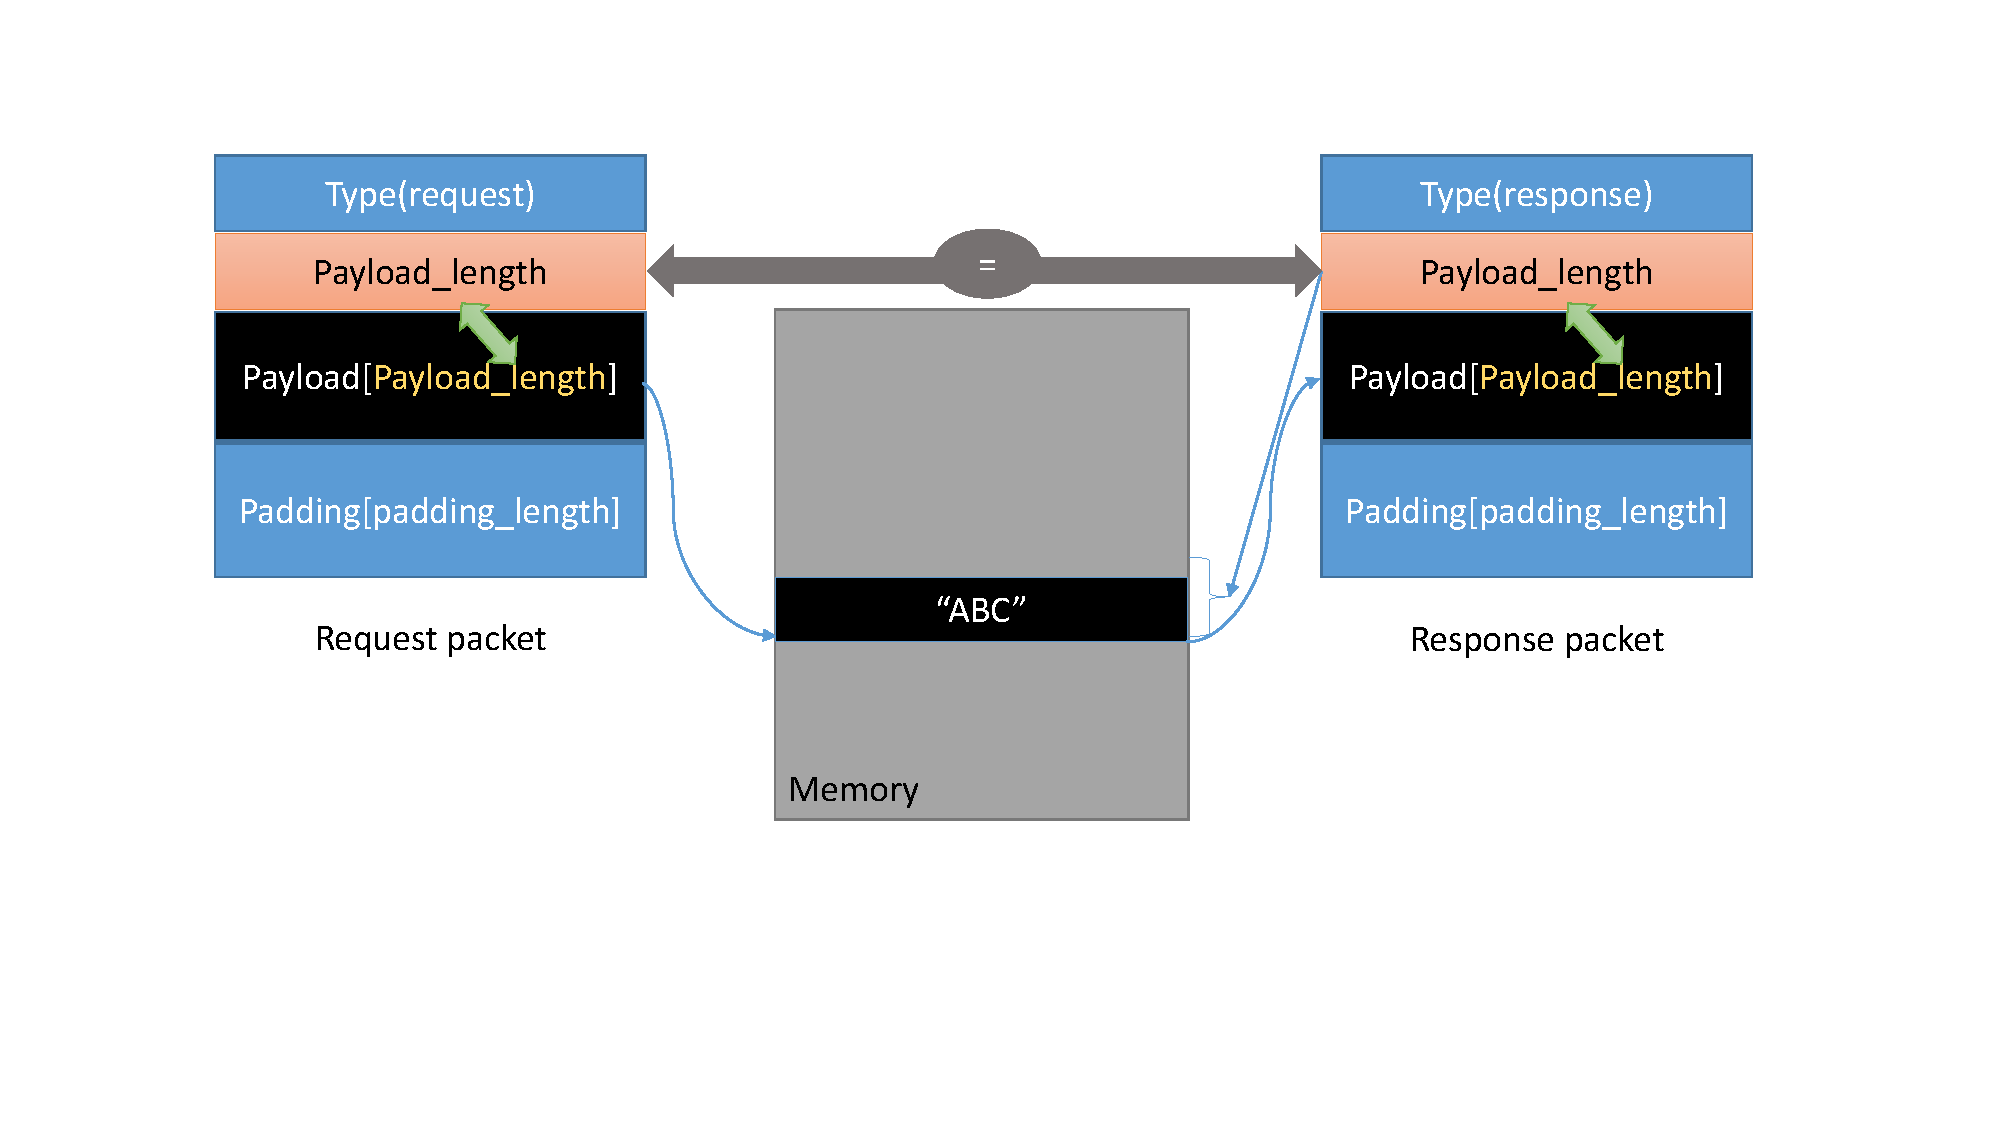
\includegraphics[width=0.8\textwidth]{\heartFigs/benign_packet.pdf}
\caption{Request Benigno de Heartbeat} 
\label{fig:benign_packet}
\end{figure}

En esta tarea, jugaremoos con el campo de longitud del request.
Primero vamos entender como se construye un paquete de respuesta Heartbeat, Figura \ref{fig:benign_packet}. Cuando llega un paquete request Heartbeat, el servidor parseará ese paquete, obtendrá el payload y el valor del \texttt{Payload\_length} (que está remarcado en la Figura \texttt{Payload\_length}). Aquí, este payload es una cadena de 3 bytes \texttt{"ABC"} y el valor de su \texttt{Payload\_length} es 3. El programa del servidor confiará ciegamente en este valor de longitud que proviene del paquete de request. Construirá el paquete de respuesta apuntando a la porción de memoria que contiene \texttt{"ABC"} y copiará los bytes del \texttt{Payload\_length} en el payload de su respuesta, de esta forma el paquete de respuesta tendrá una cadena de 3 bytes  \texttt{"ABC"}.

\begin{figure}[!htb]
\centering
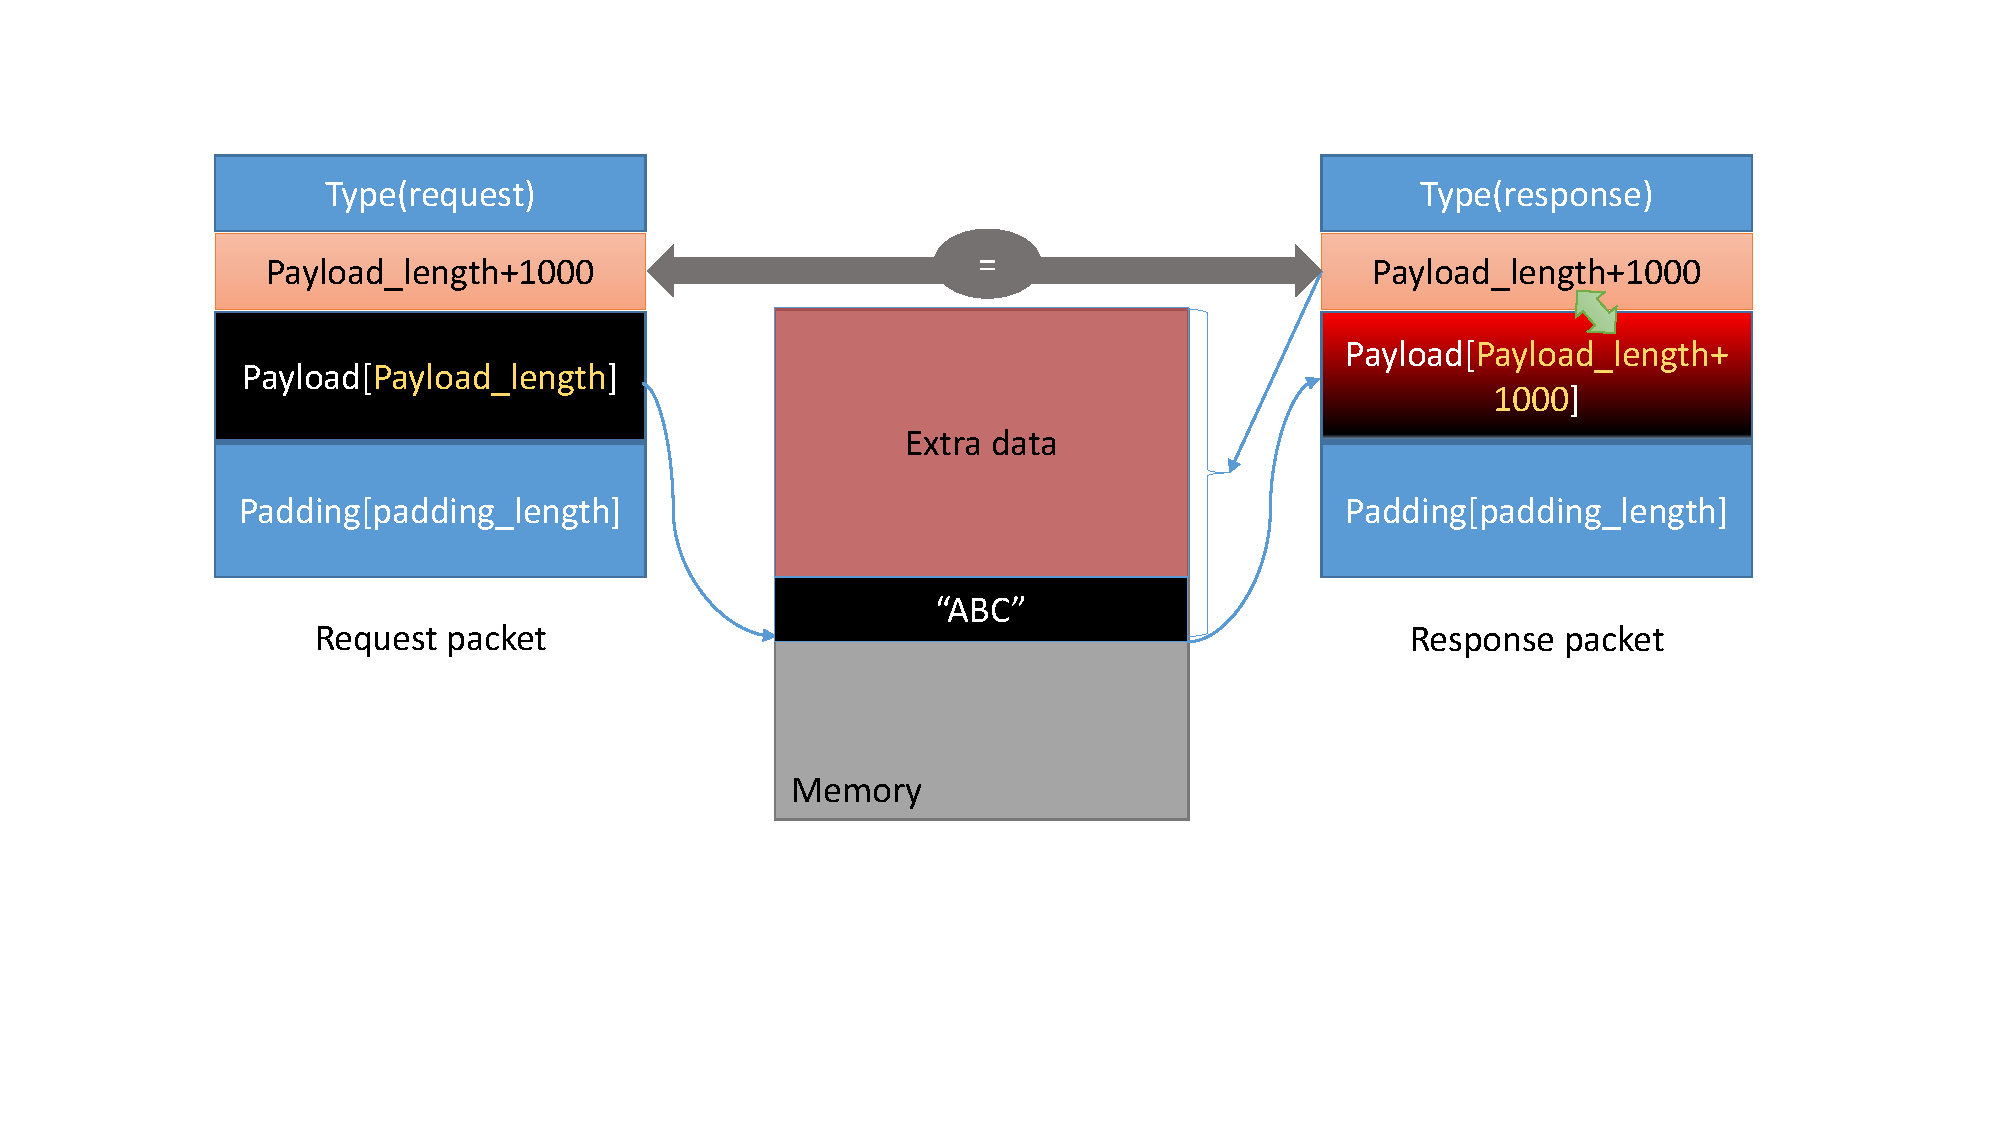
\includegraphics[width=0.8\textwidth]{\heartFigs/mal_packet.pdf}
\caption{Ataque de Heartbleed} 
\label{fig:mal_packet}
\end{figure}

Podemos lanzar el ataque Heartbleed como es mostrado en la Figura\ref{fig:mal_packet}. Usaremos el mismo payload (3 bytes) pero pondremos el valor del campo \texttt{Payload\_length} en 1003. El servidor nuevamente confiará ciegamente en el valor de \texttt{Payload\_length} al momento de construir el paquete de respuesta. Esta vez, el programa del servidor apuntara a la cadena \texttt{"ABC"} y además copiará 1003 bytes desde la memoria hacia el payload del  paquete de respuesta. Es decir ademas de copiar la cadena "ABC", se agregan en el paquete de respuesta 1000 bytes extra, que pueden contener cualquier tipo de dato que este siendo albergado en memoria en ese preciso instante, como podría ser una llave secreta, password, información de logueo, etc.

Nuestro código de ataque nos permite jugar con diferentes valores para el campo \texttt{Payload\_length}. Por defecto, el valor de este campo es un poco grande (\texttt{0x4000}), pero puede reducir su tamaño usando el parámetro  \texttt{"-l"}  (la letra L) o \texttt{"--length"}, a continuación se muestra un ejemplo:

\begin{lstlisting}
$./attack.py  www.heartbleedlabelgg.com  -l  0x015B 
$./attack.py  www.heartbleedlabelgg.com	 --length 83
\end{lstlisting}
 
Su tarea es jugar con el programa de ataque y usar diferentes longitudes de payload y después contestar las siguientes preguntas:


\begin{itemize}
  \item {\bf Pregunta 2.1:} A medida que la longitud disminuye, ¿Que diferencia puede observar?
  
  \item {\bf Pregunta 2.2:} A medida que la variable de longitud disminuye, existe un valor límite para la variable de la longitud de entrada. Por encima o por debajo de ese límite la consulta de Heartbeat recibirá un paquete de respuesta sin adjuntar ningún dato adicional (lo que significa que el request es benigno). Por favor encuentre cual es esa longitud límite. Puede que necesite intentar con varias longitudes diferentes hasta que el servidor web envíe la respuesta sin datos adicionales. Para ayudarlo con esto, cuando el número de bytes devueltos es menor que la longitud esperada, el programa imprimirá \texttt{"Server processed malformed Heartbeat, but did not return any extra data."}
\end{itemize}




% -------------------------------------------
% SUBSECTION
% ------------------------------------------- 
\subsection{Tarea 3: Protección y Arreglo del Bug}

Para arreglar la vulnerabilidad de Heartbleed, la mejor forma de hacerlo es actualizar la librería de OpenSSL a su versión más reciente. Esto se puede hacer usando los siguientes comandos.
Cabe señalar que una vez actualizada. Es difícil volver a una versión vulnerable de la librería. Asegurése de haber terminado todas las tareas previas hasta este punto antes de hacer el update. Puede realizar un snapshot de su Máquina Virtual antes de hacer el update.

\begin{lstlisting}
$ sudo apt-get update
$ sudo apt-get upgrade
\end{lstlisting}


\paragraph{Tarea 3.1} Intente lanzar el ataque una vez que haya actualizado la versión de la librería OpenSSL. Por favor describa sus observaciones.



\paragraph{Tarea 3.2} El objetivo de esta tarea es descubrir como arreglar el bug de Heartbleed en el código fuente. La siguiente estructura escrita en C (no es exactamente igual a la usada en el código) quiere mostrar el format de un paquete de request/response de Hearbeat.


\begin{lstlisting}
struct {
   HeartbeatMessageType type; // 1 byte: request or the response
   uint16 payload_length;     // 2 byte: the length of the payload
   opaque payload[HeartbeatMessage.payload_length]; 
   opaque padding[padding_length]; 
} HeartbeatMessage;
\end{lstlisting}

El primer campo (1 byte) del paquete representa el tipo de información y el segundo campo (2 bytes) es la longitud del payload, seguido por payload actual y paddings. El tamaño del payload debería de ser el mismo que el valor del campo \texttt{payload\_length} pero en un escenario de ataque, \texttt{payload\_length}  puede tener un valor diferente. El siguiente fragmento de código muestra como el servidor copia los datos del paquete de request al paquete de response.


\begin{lstlisting}[caption={Process the Heartbeat request packet and generate the response packet}, 
      label=heartbleed:source]
/* Allocate memory for the response, size is 1 byte
 * message type, plus 2 bytes payload length, plus
 * payload, plus padding
 */

unsigned int payload;
unsigned int padding = 16; /* Use minimum padding */

// Read from type field first  
hbtype = *p++;   /* After this instruction, the pointer
                  * p will point to the payload_length field *.

// Read from the payload_length field 
// from the request packet 
n2s(p, payload); /* Function n2s(p, payload) reads 16 bits
                  * from pointer p and store the value 
                  * in the INT variable "payload". */
			  
			  
pl=p; // pl points to the beginning of the payload content
			  
if (hbtype == TLS1_HB_REQUEST)
{
     unsigned char *buffer, *bp;
     int r;

     /* Allocate memory for the response, size is 1 byte
      * message type, plus 2 bytes payload length, plus
      * payload, plus padding
      */

     buffer = OPENSSL_malloc(1 + 2 + payload + padding);
     bp = buffer;

     // Enter response type, length and copy payload 
     *bp++ = TLS1_HB_RESPONSE;
     s2n(payload, bp);
        
     // copy payload 
     memcpy(bp, pl, payload); /* pl is the pointer which 
                               * points to the beginning 
	                       * of the payload content */

     bp += payload;
			    
     // Random padding
     RAND_pseudo_bytes(bp, padding);			    

     // this function will copy the 3+payload+padding bytes
     // from the buffer and put them into the heartbeat response 
     // packet to send back to the request client side.
     OPENSSL_free(buffer);
     r = ssl3_write_bytes(s, TLS1_RT_HEARTBEAT, buffer,
           3 + payload + padding); 
}
\end{lstlisting}

Por favor señale el problema del código en el Fragmento \ref{heartbleed:source} y  provea una solución para arreglar el bug de Heartbleed (es decir que modificación es necesaria para arreglar este bug). No necesita recompilar el código; solamente describa como puede solucionar el problema en su informe de laboratorio.


Además, comente sobre las siguientes discusiones de Alice, Bob y
Eva, sobre la causa fundamental de la vulnerabilidad Heartbleed:
Alice piensa que la causa fundamental es la falta de un chequeo de límites durante la copia del buffer; Bob piensa que la causa es la falta de una validación apropiada en la entrada del usuario; Eva piensa que podemos eliminar el valor de longitud del paquete para resolver todo.



% *******************************************
% SECTION
% ******************************************* 
\section{Informe del Laboratorio}

%%%%%%%%%%%%%%%%%%%%%%%%%%%%%%%%%%%%%%%%

Debe enviar un informe de laboratorio detallado, con capturas de pantalla, para describir lo que ha hecho y lo que ha observado.
También debe proporcionar una explicación a las observaciones que sean interesantes o sorprendentes.
Enumere también los fragmentos de código más importantes seguidos de una explicación. No recibirán créditos aquellos fragmentos de códigos que no sean explicados.
%%%%%%%%%%%%%%%%%%%%%%%%%%%%%%%%%%%%%%%%


% *******************************************
% SECTION
% *******************************************
\section*{Agradecimientos}

Este documento ha sido traducido al Español por Facundo Fontana




\end{document}
